\newpage
\section{Auswertung}
\label{sec:Auswertung}
% In diesem Versuch wird eine Schaltung -- Gerät 1 -- verwendet, welche aus verschiedenen Bauteilen besteht.
Die in Tabelle \ref{tab:geraet} angegebenen Werte bestimmen maßgeblich die Eigenschaften der Schaltung.

%%%%Tabelle: Gerätedaten
\begin{table}
	\centering
	\begin{tabular}{c c c}
	\toprule
	\multicolumn{3}{c}{Parameter des Schwingkreises} \\
	{Bauteil}&{Wert}&{Fehler}\\
	%{Bauteil} & {Daten} \\
	\midrule
 Induktivität $L$ & \SI{16.78}{\milli\henry} & \pm\,\SI{0.09}{\milli\henry} \\
 Kapazität $C$    & \SI{2.066}{\nano\farad}  & \pm\,\SI{0.006}{\nano\farad} \\
 Widerstand $R_1$ & \SI{67.2}{\ohm}          & \pm\,\SI{0.2}{\ohm} \\
 Widerstand $R_2$ & \SI{682}{\ohm}           & \pm\,\SI{1}{\ohm} \\
	\bottomrule
	\end{tabular}
	\caption{Daten des ersten Serienschwingkreises.}
\label{tab:geraet}
\end{table}
Da alle Größen fehlerbehaftet sind, fließen diese nach der Gaußschen Fehlerfortpflanzung 
\begin{equation}
\Delta{u}=\sqrt{\biggl(\frac{\mathup{d}u}{\mathup{d}v}\Delta{v}\biggr)²+\biggl(\frac{\mathup{d}u}{\mathup{d}w}\Delta{w}\biggr)²}
%\label{eq:gauss}
\end{equation}
in die folgenden Rechnungen ein.
% Alle Grafiken und Ausgleichsrechnungen werden mit PROGRAMM ausgeführt.
\subsection{Zeitabhängigkeit der Amplitude einer gedämpften Schwingung}

%%%%%%%%%Schwingfall Plot
%%%%%%%%Tabelle: Extremwerte der Spannung
\begin{table}
	\centering
	\begin{tabular}{S[table-format=3.0] S[table-format=2.2] S[table-format=3.0] S[table-format=2.2]}
	\toprule
	{$t\:/{\si{\micro\second}}$} & {$U_\mathup{C,min}\:/{\si{\volt}}$} &{$t\:/{\si{\micro\second}}$}& {$U_\mathup{C,max}\:/{\si{\volt}}$} \\
	\midrule
 42 & 62.60 &  23 & -67.00\\
 80 & 54.60 &  61 & -57.40\\
117 & 45.80 &  98 & -49.40\\
155 & 39.40 & 136 & -42.20\\
193 & 34.60 & 175 & -36.60\\
232 & 29.80 & 212 & -31.00\\
269 & 25.00 & 250 & -27.00\\
306 & 21.00 & 288 & -23.80\\
346 & 19.40 & 327 & -20.60\\
381 & 15.40 & 363 & -17.40\\
421 & 13.80 & 402 & -15.00\\
457 & 11.40 & 438 & -13.40\\
	\bottomrule
	\end{tabular}
	\caption{Extrema der Spannungswerte.}
	\label{tab:extrema}
\end{table}

In Abbildung \ref{schwingfall} ist die Amplitude der Kondensatorspannung $U_\mathup{C}$ gegen die Zeit $t$ aufgetragen, nachdem der Stromkreis durch einen elektrischen Impuls zur Schwingung angeregt wurde.
Mit den eingezeichneten Extremwerten der Spannung, angegeben in Tabelle \ref{tab:extrema}, kann die Schwingungskurve berechnet werden.
Die Einhüllende, die nur die Minima und Maxima mit der Schwingkurve gemein hat, zeigt den für den Schwingfall typischen zeitlichen Verlauf der Spannung. 
Diese nimmt exponentiell ab.
\begin{figure}[h]
		\centering
		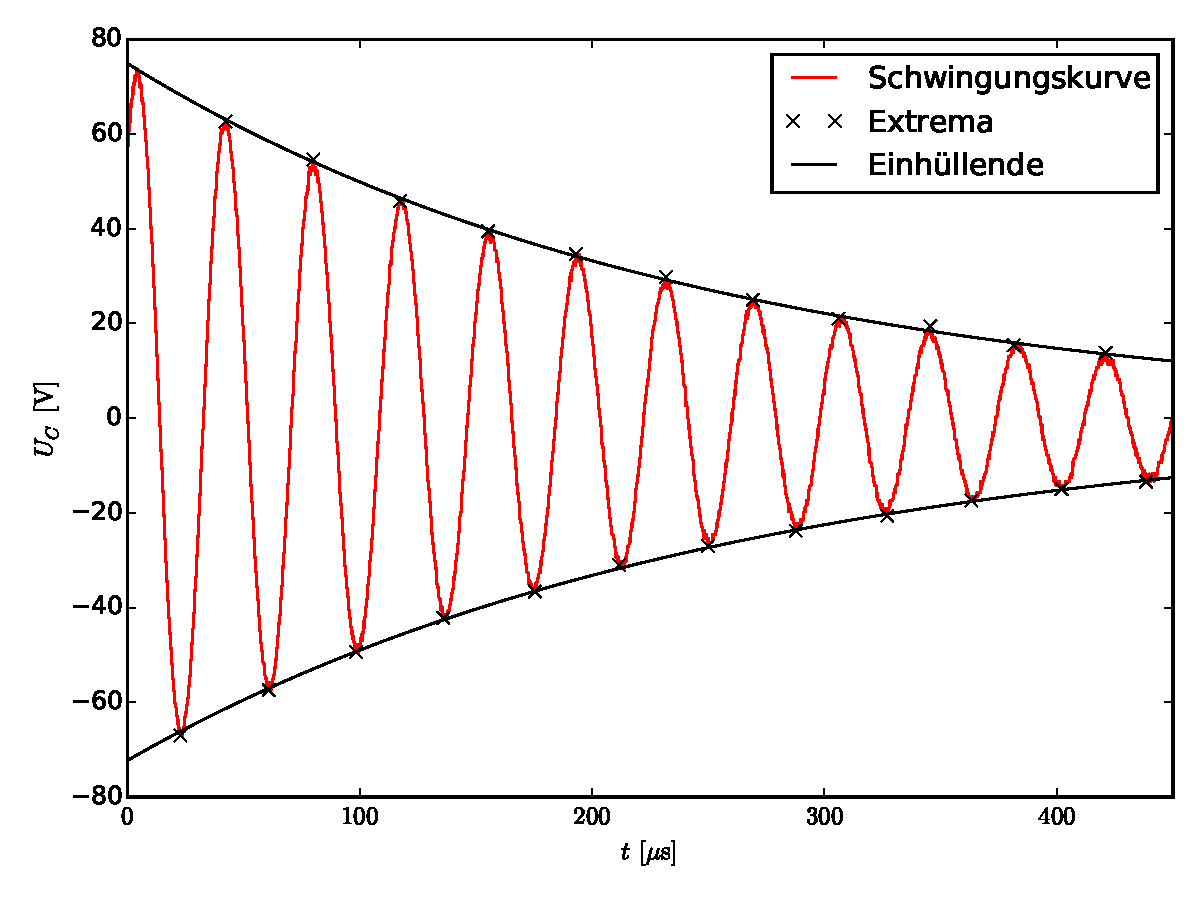
\includegraphics[width=\textwidth]{build/plot_schwingungskurve.pdf}
		\caption{Verhalten der Spannung für den Schwingfall. \cite{matplotlib}}
\label{schwingfall}
\end{figure}
Noch deutlicher wird es, wenn die Extremwerte halblogarithmisch aufgetragen werden. Dafür werden die Minima an der $t$-Achse gespiegelt. Ein linearer Zusammenhang ist erkennbar.
%%%%%%%Schwingfall, logarithmischer Plot
\begin{figure}[h]
		\centering
		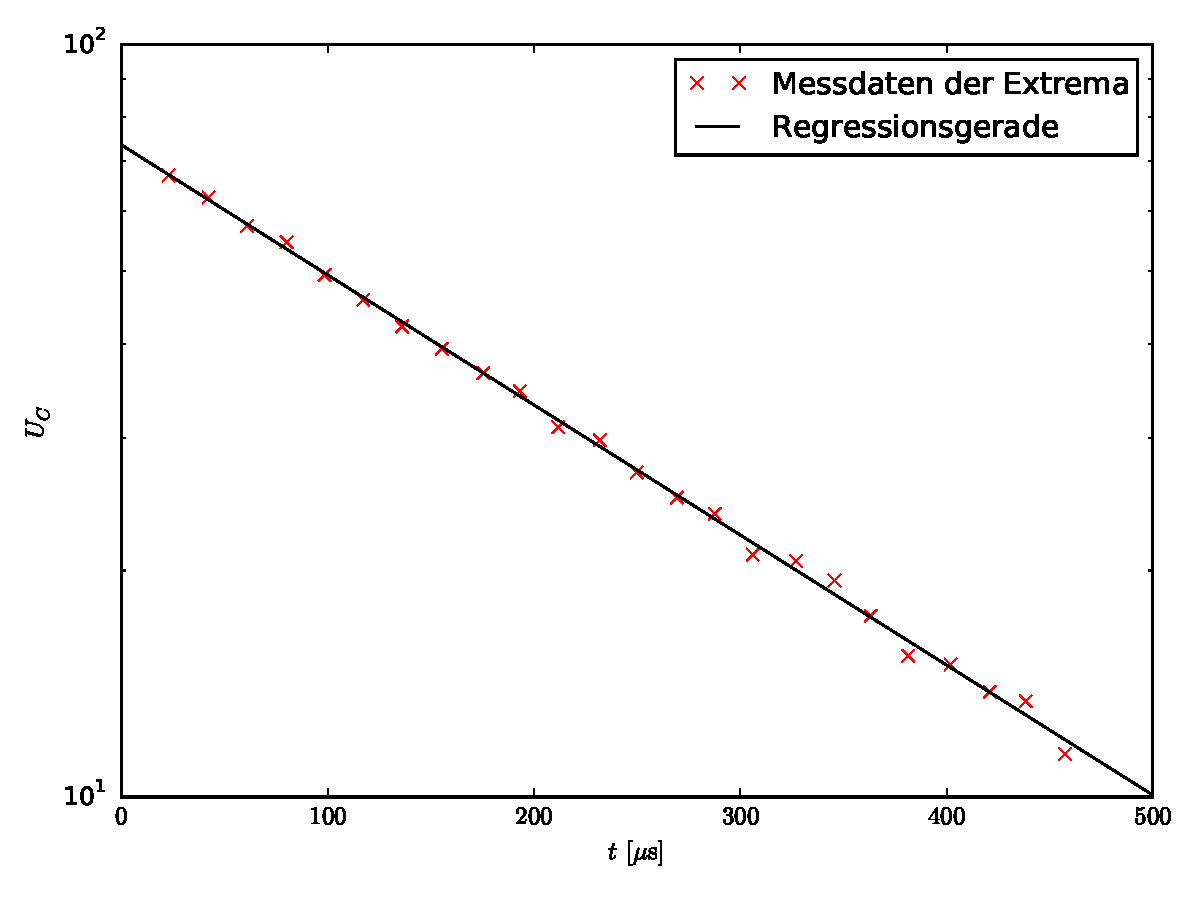
\includegraphics[width=\textwidth]{build/plot_einhuellende_semilog.pdf}
		\caption{Einhüllende der Schwingungskurve, aufgetragen auf halblogarithmischer Skala. \cite{matplotlib}}
\end{figure}
Durch lineare Regression kann mit
\begin{equation}
\ln{U_\mathup{C}}(t)=\bigl(\underbrace{-\frac{R}{2L}}_m\bigr)\cdot t +b
\end{equation}
eine Ausgleichsgerade 
\begin{equation}
g(t)=(-3978.365\pm 36.562)\frac{1}{s} t + (4.298\pm0.010)
\end{equation}
durch die Messpunkte gelegt werden. 
$m$ ist dabei die Steigung der Geraden und $b$ der y-Achsenabschnitt.
Damit lässt sich $R_\mathup{eff}=\sfrac{\mathup{-2m}}{\mathup{L}}=(134\pm1)\,\si\ohm$, der für die in der Schaltung auftretende Dämpfungswiderstand, berechnen. 

Die Abklingdauer $T_\mathup{ex}$ wird aus dem negativen Kehrwert der Steigung $m$ gebildet, sodass $T_\mathup{ex}=(251\pm2)\,\si{\micro{\second}}$ ist.
Der theoretische Wert nach Gleichung \eqref{eq:abkling} ergibt sich zu \\$T_\mathup{ex,t}=(499\pm3)\,\si{\micro{\second}}$.


%%%%%%%%%%%%%%%%%%%%neues Unterkapitel
\subsection{Aperiodischer Grenzfall im gedämpften Schwingkreis}
Der Spannungsverlauf für den aperiodischen Grenzfall wird durch einen Widerstand von $R_\mathup{ap}\approx4500\,\si\ohm$ realisiert. 
Der Theoriewert ergibt sich aus der Formel $R_\mathup{ap,t}=2\sqrt\frac{L}{C}$ zu $R_\mathup{ap,t}=(5700\pm20)\,\si\ohm$
%%%%%%%%%%%%%%%%%%%%%%%%%%%%%BERICHTIGUNG
% $R_\mathup{ap,t}=(5700\pm15)\,\si\ohm$ ist anscheinend falsch gerundet, der Fehler ist "anders". Ist das nun so richtig?
 Zum Vergleich sind ebenfalls Schwing- und Kriechfall dargestellt.
\newpage
%%%%%%%%%%%%%%%%%Aperiodischer Grenzfall, Screenshot
\begin{figure}[h]
		\centering
		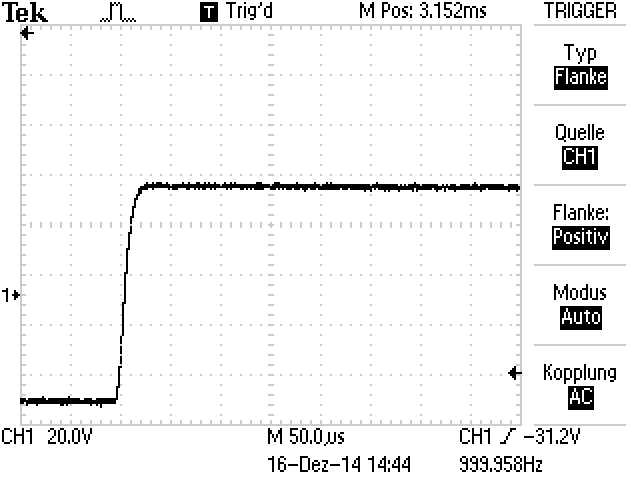
\includegraphics[width=0.8\textwidth]{Bilder/Aperiodischer.JPG}
		\caption{Screenshot des aperiodischen Grenzfalls.}
\end{figure}

\begin{figure}[hbp]
	\centering
	\begin{subfigure}{0.4\textwidth}
		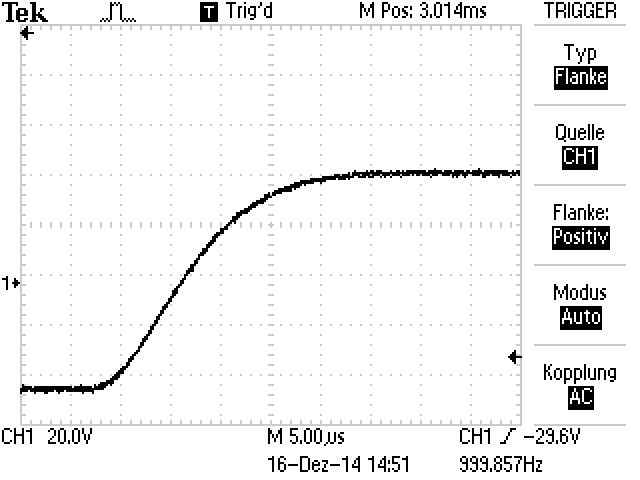
\includegraphics[width=\textwidth]{Bilder/Kriechfall1.JPG}
		\caption{Kriechfall.}
	\end{subfigure}
	\begin{subfigure}{0.4\textwidth}
		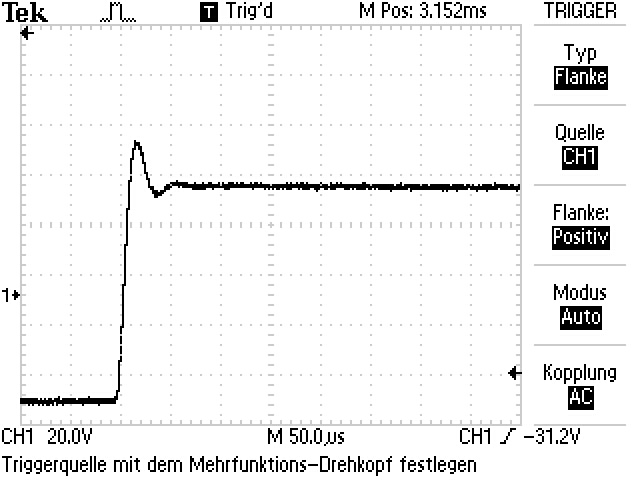
\includegraphics[width=\textwidth]{Bilder/Schwingfall.JPG}
		\caption{Schwingfall.}
	\end{subfigure}
	\caption{Schwing- und Kriechfall zum Vergleich.}
	\label{fig:faelle}
\end{figure}
\newpage
%%%%%%%%%%%%%%%%%%%%%%%%%%%%%%%%neues Unterkapitel
\subsection{Frequenzabhängigkeit der Kondensatorspannung}
%%%%%tabelle: kondensatorspannung,, frequenzabh.
\begin{table}
	\centering
\setlength{\tabcolsep}{2mm}
\begin{tabular}{cc}
	\begin{tabular}{S[table-format=2.1] S[table-format=3.0] S[table-format=2.1] }
	\toprule
	{$f\:/{\si{\kilo\hertz}}$} & {$U_\mathup{C}\:/{\si{\volt}}$} & {$U_\mathup{0}\:/{\si{\volt}}$} \\
	\midrule

10.0 &  48 & 44.0\\
11.0 &  52 & 44.0\\
12.0 &  54 & 44.0\\
13.0 &  58 & 44.0\\
14.0 &  60 & 44.0\\
15.0 &  64 & 44.0\\
16.0 &  66 & 44.0\\
17.0 &  72 & 44.0\\
18.0 &  78 & 44.0\\
19.0 &  84 & 44.0\\
20.0 &  92 & 43.2\\
20.5 &  96 & 43.2\\
21.0 & 102 & 43.2\\
21.5 & 108 & 43.2\\
22.0 & 114 & 43.2\\
22.5 & 120 & 42.4\\
23.0 & 128 & 42.4\\
23.5 & 136 & 42.4\\
24.0 & 142 & 42.4\\
24.5 & 150 & 42.4\\
25.0 & 156 & 41.6\\
25.5 & 158 & 41.6\\
26.0 & 160 & 41.6\\
26.5 & 158 & 40.8\\
27.0 & 152 & 40.8\\
27.5 & 144 & 40.8\\
\bottomrule
	\end{tabular}
&	
	\begin{tabular}{S[table-format=2.1] S[table-format=3.0] S[table-format=2.1] }
	\toprule
	{$f\:/{\si{\kilo\hertz}}$} & {$U_\mathup{C}\:/{\si{\volt}}$} & {$U_\mathup{0}\:/{\si{\volt}}$} \\
	\midrule
28.0 &  136.0   & 40.8\\
28.5 &  128.0 	& 41.6\\
29.0 &  118.0 	& 41.6\\
29.5 &  108.0 	& 41.6\\
30.0 &  100.0 	& 41.6\\
30.5 &   94.0 	& 41.6\\
31.0 &   88.0 	& 42.4\\
32.0 &   76.0 	& 43.2\\
33.0 &   66.0 	& 43.2\\
34.0 &   56.0 	& 43.2\\
35.0 &	 49.0	& 43.2\\
36.0 &	 44.8 	& 43.2\\
37.0 &	 40.8 	& 43.2\\
38.0 &	 36.8 	& 43.2\\
39.0 &	 33.6 	& 43.2\\
40.0 &	 30.8 	& 43.2\\
41.0 &	 28.4 	& 43.2\\
42.0 &	 26.4 	& 43.2\\
43.0 &	 24.4 	& 43.2\\
44.0 &	 22.8 	& 43.2\\
45.0 &	 21.6 	& 43.2\\
46.0 &	 20.0 	& 43.2\\
47.0 &	 18.8 	& 43.2\\
48.0 &	 18.0 	& 43.2\\
49.0 &	 16.8 	& 43.2\\
50.0 &	 16.0 	& 43.2\\
\bottomrule
\end{tabular}
\end{tabular}
	\caption{Messdaten der Kondensator- und Generatorspannung zu verschiedenen Frequenzen.}
	\label{tab:f_U}
\end{table}
Das Verhältnis der Spannungen $\frac{U_\mathup{C}}{U_0}$, deren Werte in Tabelle \ref{tab:f_U} gelistet sind, wird gegen die Frequenz $f$ halblogarithmisch aufgetragen. 
Es ergibt sich eine Resonanzkurve, deren Maximum bei $f_\mathup{res}\approx26\,\si{\kilo\hertz}$ liegt.
 Bei dieser Frequenz ist die Kondensatorspannung um ein Vielfaches größer als die angelegte Spannung $U_0$. 
Für die Resonanzüberhöhung  $q=\frac{U_\mathup{C,max}}{U_0}$, auch Güte genannt, ergibt sich aus der Messung der Wert $q=5.556$ bei einer maximalen Kondensatorspannung $U_\mathup{C,max}=160\,\si\volt$. 
%%BERICHTIGUNG von 5\pm1 zu 4.18\pm 0.01
Theoretisch ergibt sich $q_\mathup{t}=\frac{1}{R_2}\sqrt{\frac{L}{C}}$ zu $q_\mathup{t}=4.18\pm0.01$.

Für die Breite der Resonanzkurve werden die Grenzfrequenzen $f_\pm=\frac{U_\mathup{C,max}}{\sqrt{2}}$ berechnet. Es ergeben sich zwei Lösungen, deren Differenz $f_+-f_-$ anschließend gebildet wird. 
Damit sind $f_+=29\,\si{\kilo\hertz}$, $f_-=22\,\si{\kilo\hertz}$ und $\Delta{f}=7\,\si{\kilo\hertz}$. 
Die theoretische Resonanzbreite ist $\Delta{f_\mathup{t}}=\frac{R_2}{L\cdot2\pi}=(6.5\pm0.04)\,\si{\kilo\hertz}$. 
\begin{figure}[h]
		\centering
		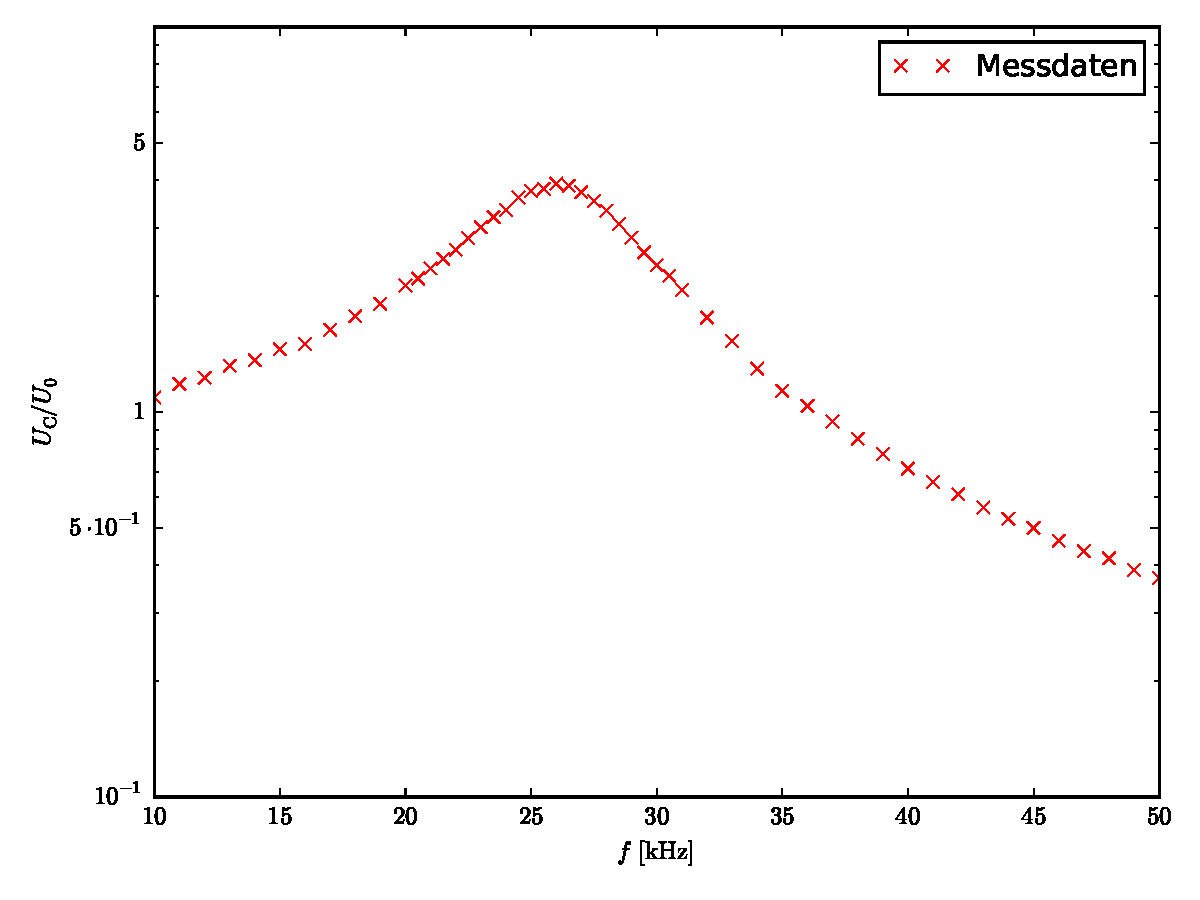
\includegraphics[width=0.8\textwidth]{build/plot_amplitude_semilog.pdf}
		\caption{Resonanzkurve der erzwungenen Schwingungen in halblogarithmischer Skala.\cite{matplotlib}}
\end{figure}
\begin{figure}[h]
		\centering
		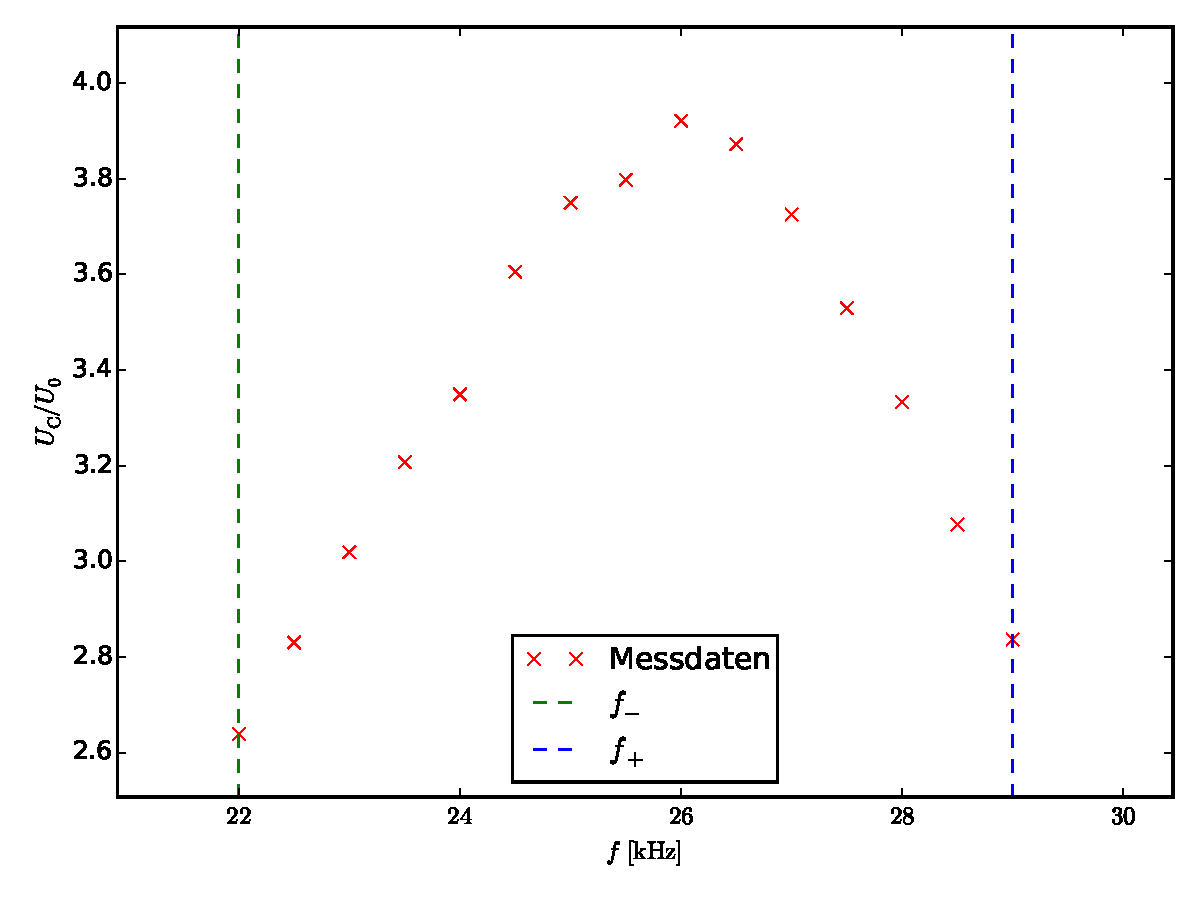
\includegraphics[width=0.8\textwidth]{build/plot_amplitude_linear.pdf}
		\caption{Lineare Darstellung des Spannungsverhältnissen in Abhängigkeit der Frequenz zwischen den Grenzfrequenzen.\cite{matplotlib}}
\end{figure}

%%%%%%%%%%%%%%%%%%%neues Unterkapitel
\subsection{Frequenzabhängigkeit der Phasendifferenz}
In Tabelle \ref{tab:f_t} ist die frequenzabhängige Zeitdifferenz $\Delta{t}$ zwischen den Nulldurchgängen der Sinusspannung des Frequenzgenerators $U(t)$ und der Kondensatorspannung $U_\mathup{C}(\omega, t)$ aufgetragen. 
\begin{table}	
\centering
\setlength{\tabcolsep}{2mm}
\begin{tabular}{cc}
	\begin{tabular}{S[table-format=2.1] S[table-format=3.0] S[table-format=2.1] }
	\toprule
	{$f\:/{\si{\kilo\hertz}}$} & {$\Delta{t}\:/{\si{\micro\second}}$} \\
	\midrule
10.0 &  2.0\\
11.0 &  2.0\\
12.0 &  2.0\\
13.0 &  2.4\\
14.0 &  2.4\\
15.0 &  2.8\\
16.0 &  2.8\\
17.0 &  2.8\\
18.0 &  3.2\\
19.0 &  3.2\\
20.0 &  3.6\\
20.5 &  4.0\\
21.0 &  4.0\\
21.5 &  4.2\\
22.0 &  4.6\\
22.5 &  4.8\\
23.0 &  5.4\\
23.5 &  5.4\\
24.0 &  6.0\\
24.5 &  6.4\\
25.0 &  7.6\\
25.5 &  8.2\\
26.0 &  9.2\\
26.5 &  9.6\\
27.0 & 10.4\\
27.5 & 11.2\\
\bottomrule
	\end{tabular}
&	
	\begin{tabular}{S[table-format=2.1] S[table-format=3.0] S[table-format=2.1] }
	\toprule
	{$f\:/{\si{\kilo\hertz}}$} & {$\Delta{t}\:/{\si{\micro\second}}$} \\
	\midrule
28.0 &  11.6\\
28.5 &  11.8\\
29.0 &  12.4\\
29.5 &  12.2\\
30.0 &  12.8\\
30.5 &  13.0\\
31.0 &  12.4\\
32.0 &  12.6\\
33.0 &  12.4\\
34.0 &  12.6\\
35.0 &	12.2\\
36.0 &	11.8\\
37.0 &	11.6\\
38.0 &	12.0\\
39.0 &	11.6\\
40.0 &	11.4\\
41.0 &	11.4\\
42.0 &	11.2\\
43.0 &	11.0\\
44.0 &	10.8\\
45.0 &	10.4\\
46.0 &	10.2\\
47.0 &	10.2\\
48.0 &	 9.6\\
49.0 &	 9.6\\
50.0 &	 9.6\\
\bottomrule
\end{tabular}
\end{tabular}
\caption{Messdaten der Phasendifferenz zu verschiedenen Frequenzen.}
	\label{tab:f_t}
\end{table}
Die Phase $\varphi$ ist in Abbildung \ref{fig:phase} gegen die Frequenz aufgetragen. Phase und Zeitdifferenz sind über $\varphi(f)=2\pi\Delta{t}f$ verknüpft. Für große Frequenzen nähert sich die Phase dem stationären Wert $\pi$ an. 

In der Abbildung \ref{fig:phase} ist zu erkennen, dass die Phasendifferenz erst langsam wächst, um mit zunehmender Frequenz schneller anzusteigen. 
Je näher die Frequenz an der Resonanzfrequenz liegt, desto steiler ist die Kurve. 
Es ist ersichtlich, dass um die Resonanzfrequenz  $f_\mathup{res}\approx25\,\si{\kilo\hertz}$ die Kurve als linear angenähert werden kann, wie in Abbildung \ref{fig:phase_lin} gezeigt. 
Die Linearität erstreckt sich über $\frac{\pi}{2}\leq\varphi\leq\frac{3\pi}{2}$, was den Frequenzen $f_1=22\,\si{\kilo\hertz}$ und $f_2=30\,\si{\kilo\hertz}$ entspricht.
Der Verlauf scheint ein logistisches Wachstum zu beschreiben.
\begin{figure}[h]
		\centering
		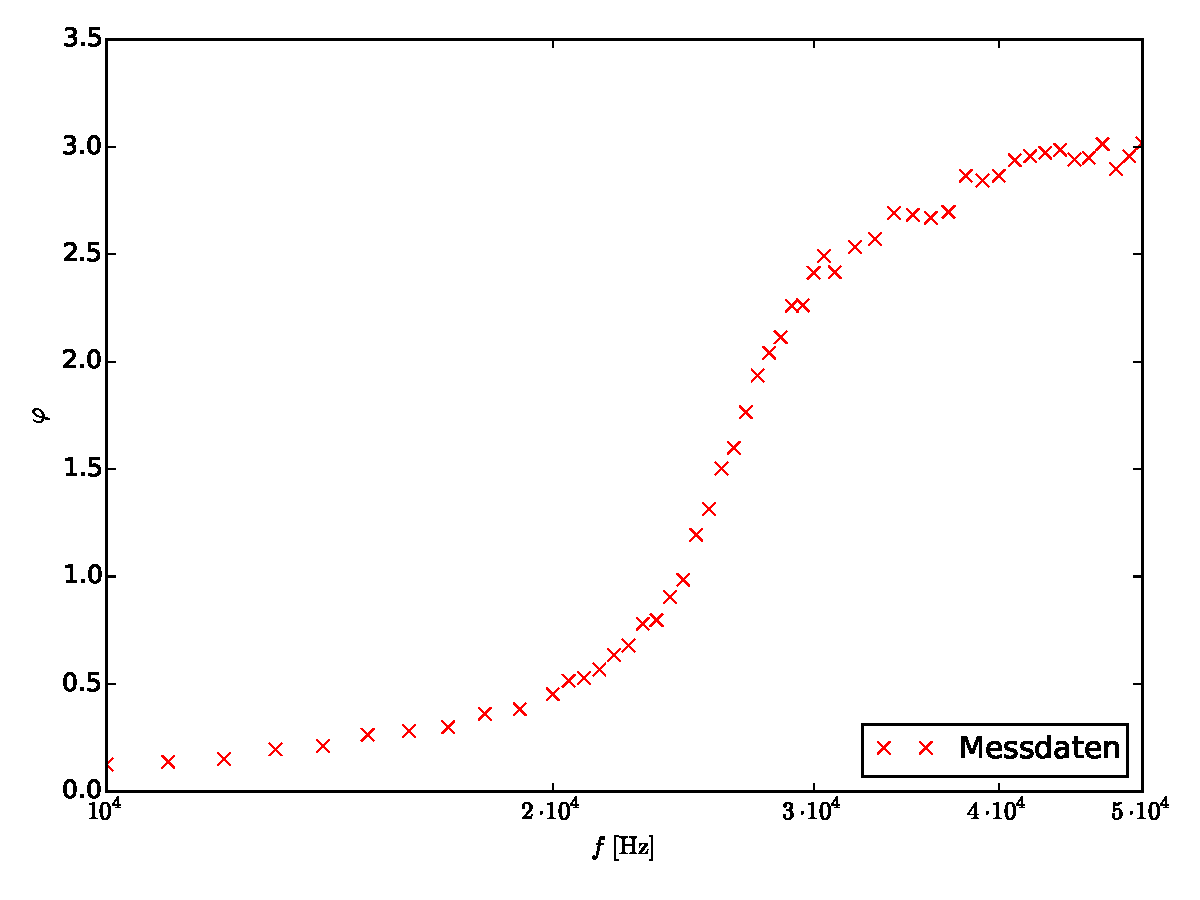
\includegraphics[width=0.8\textwidth]{build/plot_phase.pdf}
		\caption{Messdaten der Phasendifferenz zu verschiedenen Frequenzen. \cite{matplotlib}}
\label{fig:phase}
\end{figure}
\begin{figure}[h]
		\centering
		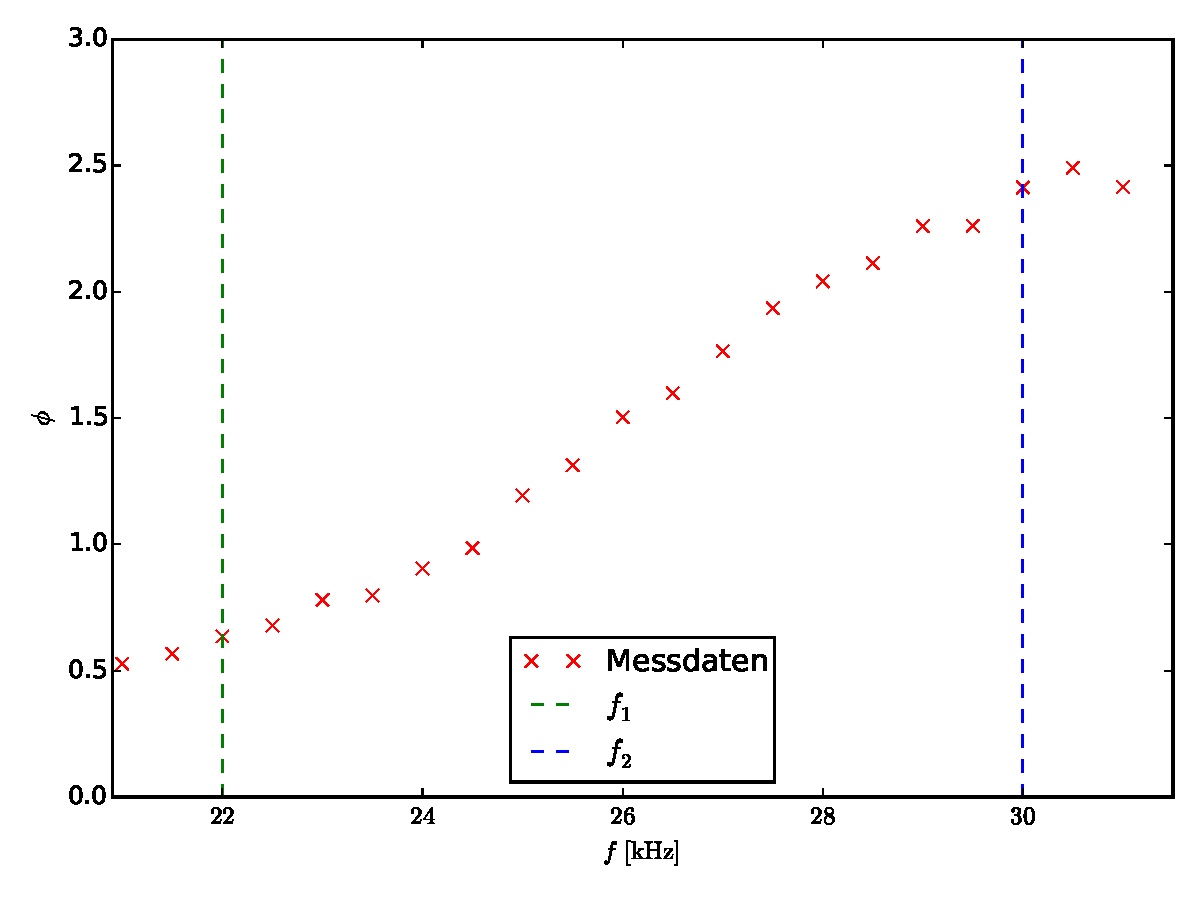
\includegraphics[width=0.8\textwidth]{build/plot_phase_linear.pdf}
		\caption{Messdaten der Phasendifferenz zu verschiedenen Frequenzen, linearer Anteil. \cite{matplotlib}}
\label{fig:phase_lin}
\end{figure}
